\documentclass[14pt]{article}
\usepackage{polski}
\usepackage[utf8]{inputenc}
\usepackage{amsmath}
\usepackage{amsfonts}
\usepackage{tabto,lipsum}
\usepackage{xcolor}
\usepackage{shadowtext}
\usepackage{hyperref}
\hypersetup{%
  colorlinks=false,% hyperlinks will be black
  linkbordercolor=red,% hyperlink borders will be red
  pdfborderstyle={/S/U/W 1}% border style will be underline of width 1pt
}
\usepackage[margin=3cm]{geometry}
\usepackage{algpseudocode}
\usepackage{algorithm}

\PassOptionsToPackage{usenames,dvipsnames,svgnames}{xcolor}
\usepackage{tikz}
\usetikzlibrary{arrows,positioning,automata}

\linespread{1.3}

\title{Lista 6}
\author{Zadanie 1}
\date{------------}

\begin{document}

\maketitle

\section{Problem}

Rozważamy skierowany graf acykliczny (\href{https://en.wikipedia.org/wiki/Directed_acyclic_graph}{DAG}) $G=(V,E,f)$ gdzie każda krawędź $e \in E$ ma swój koszt określany przez funkcję $f: V\times V \to \mathbb{R}$. Chcemy znaleźć wszystkie najkrótsze („najtańsze”) ścieżki od źródła ($v_s \in V$ t. że $\deg^-(v_s) = 0$) do pozostałych wierzchołków $V\setminus\{v_s\}$.

W przykładzie poniżej wierzchołkiem źródłowym jest wierzchołek $D$.

\begin{figure}[!h]
\centering
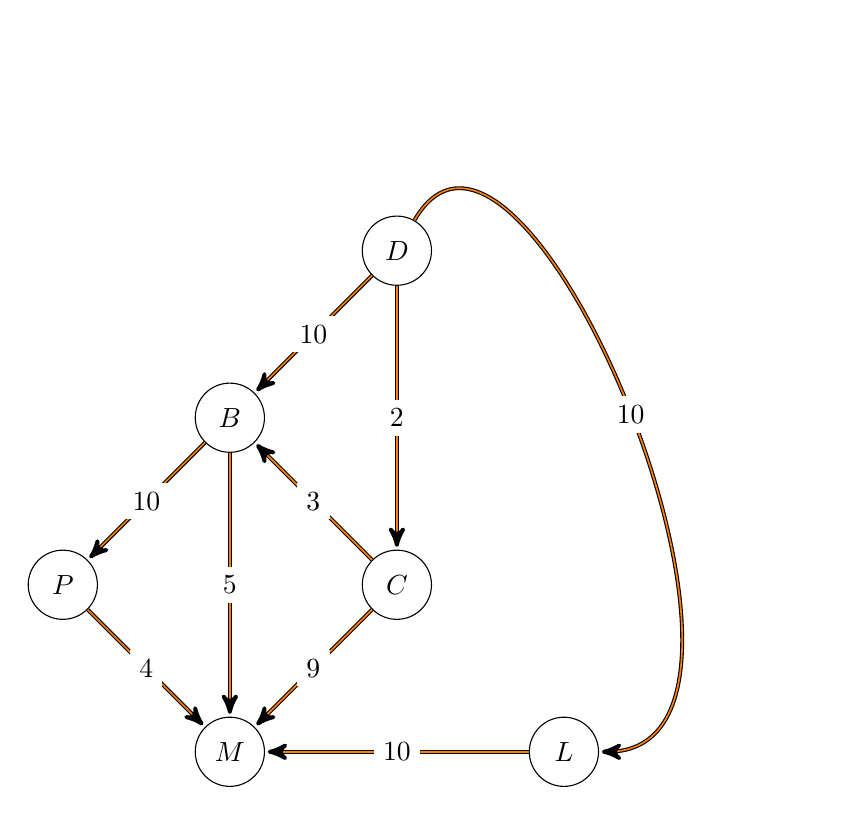
\begin{tikzpicture}[>=stealth',shorten >=1pt,node distance=3cm,on grid,initial/.style    ={}]
  \node[state]          (P)                        {$P$};
  \node[state]          (B) [above right =of P]    {$B$};
  \node[state]          (M) [below right =of P]    {$M$};
  \node[state]          (D) [above right =of B]    {$D$};
  \node[state]          (C) [below right =of B]    {$C$};
  \node[state]          (L) [below right =of C]    {$L$};
\tikzset{mystyle/.style={->,double=orange}}
\tikzset{every node/.style={fill=white}}
\path (C)     edge [mystyle]    node   {$3$} (B)
      (D)     edge [mystyle]    node   {$10$} (B)
      (L)     edge [mystyle]    node   {$10$} (M)
      (B)     edge [mystyle]    node   {$10$} (P);
\tikzset{mystyle/.style={->,double=orange}}
\path (P)     edge [mystyle]   node   {$4$} (M)
      (C)     edge [mystyle]   node   {$9$} (M)
      (D)     edge [mystyle]   node   {$2$} (C)
      (B)     edge [mystyle]   node   {$5$} (M);
\tikzset{mystyle/.style={->,relative=false,in=0,out=60,double=orange}}
\path (D)     edge [mystyle]   node   {$10$} (L);
\end{tikzpicture}
\caption{Przykładowy DAG}
\label{fig:example-dag}
\end{figure}

\section{Concept}

Użyjemy tutaj metodologii programowania dynamicznego. Zapamiętujemy każdą nowo odkrytą najkrótszą ścieżkę pomiędzy danymi wierzchołkami, a podczas dalszego znajdowania ścieżek wykorzystujemy tę wiedzę, którą już mamy.

\section{Rozwiązanie}

Najpierw musimy ustalić kolejność, według której będziemy przeglądać wierzchołki. Wierzchołki grafu wejściowego sortujemy topologicznie względem wierzchołka startowego. Użyjemy tutaj \href{https://en.wikipedia.org/wiki/Topological_sorting#Kahn's_algorithm}{algorytmu Kahn'a}:

\begin{algorithm}
  \caption{Algorytm Kahn'a}
  \label{kahn}
  \begin{algorithmic}[1]
    \State $L \gets [~]$
    \State $S \gets \{s\}$

    \While{$S \neq \emptyset$}:
      \State remove a node $n$ from $S$
      \State $L \gets \texttt{concat}(L, [n])$
      \For{\textbf{each} node $m$ with an edge $e$ from $n$ to $m$}:
        \State remove edge $e$ from the graph
        \If{$\deg^-(m) = 0$}:
          \State insert $m$ into $S$
        \EndIf
      \EndFor
    \EndWhile
  \end{algorithmic}
\end{algorithm}
Złożoność obliczeniowa powyższego algorytmu wynosi $O(|V| + |E|)$. Algorytm Kahn'a daje nam „zlinearyzowany” graf, po którym możemy szukać najkrótszych ścieżek pomiędzy $v_s$ a pozostałymi wierzchołkami.

Zdefiniujmy funkcję zwracającą nam indeksy wszystkich wierzchołków sąsiednich dla danego $v_k \in V$:
$$
\mathcal{N}(k) = \{j: \forall(v_j,v_k) \in E\}.
$$

Nasze poszukiwania zaczynamy od inicjalizacji tablicy odległości pomiędzy wszystkimi wierzchołkami $V$ a wierzchołkiem $v_s$.
Tablicę odległości $d[0,\dots,|V|]$ wypełniamy wartościami $\infty$, przy czym $d[s] = 0$. Wówczas $\forall_{i\in\{0,\dots,|V|\}}~ d[i]$ określa odległość pomiędzy wierzchołkiem źródłowym $v_s$ a wierzchołkiem $v_i$.

Oprócz tablicy $d$ musimy przechowywać numery indeksów wierzchołków, które tworzą znalezioną ścieżkę z $v_s$ do $v_i$. Stworzymy listę list, którą nazwiemy $r$, gdzie $r[i]$ to lista indeksów wierzchołków, które tworzą najkrótszą ścieżką pomiędzy $v_s$ a $v_i$.

\begin{algorithm}[H]
  \begin{algorithmic}[1]
    \State $d \gets [\infty,\dots,\infty]$
    \State $d[s] \gets 0$
    \State $r \gets \big[~[~],~\dots,~[~]~\big]$
    \For{\textbf{each} $i$ in $\{i: v_i \in V\}$ in linearized order}:
      \For{\textbf{each} $j$ in $\mathcal{N}(i)$}:
        \If{$d[i] > d[j] + f(j,i)$}:
          \State $d[i] \gets d[j] + f(j,i)$
          \State $r[i] \gets \texttt{concat}(r[j], [i])$
        \EndIf
      \EndFor
    \EndFor
  \end{algorithmic}
\end{algorithm}

W linijkach 6-9 sprawdzamy, czy nie ma „tańszej” drogi z wierzchołka $v_s$ do wierzchołka $v_i$. Złożoność obliczeniowa powyższego algorytmu wynosi $O(|E|)$, ponieważ w pętli rozważamy koszty powstałe dla każdej krawędzi w grafie.

\end{document}
